\chapter{Expertensysteme}
\label{chap:experten_systeme}

Bei Expertensystemen handelt es sich um Systeme zur Wissensrepräsentation, welche in einem sehr eingeschränkten (Teil-) Gebiet die Leistung eines menschlichen Experten ersetzen  oder diese sogar übertreffen können. Entwicklung und Erfolg von Expertensystemen führten zu einem standardisierten Prozess der Wissensdarstellung und zu Ontologien. Dies vereinfachte die Entwicklung von Expertensystemen in neuen, unerforschten Themengebieten erheblich (vgl.~\cite[S. 257]{russel}).

\section{Komponenten}
\label{sec:experten_systeme_komponenten}
Um ein Expertensystem aufbauen zu können, muss zuerst das Wissen über einen Problembereich formalisiert werden.

Die dazu benötigten Komponenten sind:
\begin{itemize}
    \item Eine Wissensdatenbank, welche die Fakten des Problembereiches in formaler Sprache enthält
    \item Ein Verarbeitungsmechanismus zum automatischen Ziehen von Schlüssen (Inferenz-Maschine)
\end{itemize}

\begin{figure}[htbp]
\centering \rotatebox{0}{\scalebox{0.5}[0.5]{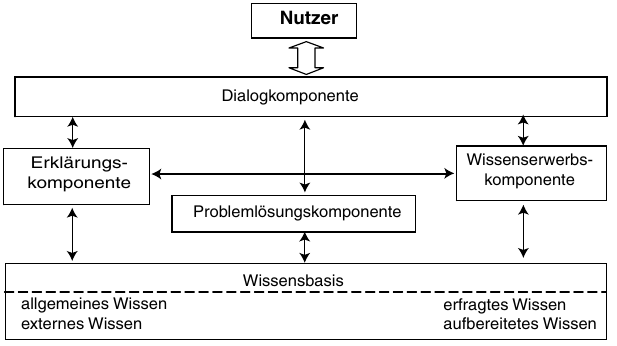
\includegraphics{bilder/aufbau_expertensysteme.png}}}
\caption{Aufbau eines Expertensystems.\label{fig:aufbau_expertensysteme}\protect\footnotemark}
\end{figure}
\footnotetext{Eigene Darstellung mittels yEd, basierend auf~\cite[S. 23]{laemmel}}

(vgl.~\cite[S. 23]{laemmel})

\newpage

\section{Problemlösung}
\label{sec:experten_systeme_problemloesung}
Bei der Problemlösung, wird typischerweise in folgenden Schritten vorgegangen:
\begin{itemize}
    \item Charakterisierung der Problemdomäne
    \item Symbolische Repräsentation der Objekte
    \item Eingabe des Wissens in den Computer
    \item Stellen von Fragen
    \item Interpretation der Antworten
\end{itemize}

Für die symbolische Repräsentation der Objekte ist es notwendig, eine geeignete Sprache zu wählen. Diese Sprache kann beispielsweise aus mathematischen Relationen oder Logik bestehen, oder eine Programmiersprache sein.

In der Informatik wird das Wissen über ein Problem üblicherweise direkt mittels Lösungsalgorithmen programmiert. Bei der künstlichen Intelligenz hingegen, wird das Wissen von der Verarbeitungskomponente getrennt dargestellt. Dies hat den Vorteil, dass die Wissensbasis jederzeit ausgewechselt, die Verarbeitungskomponente jedoch bestehen bleiben kann. Ein Programm in Form eines Expertensystems kann somit also für unterschiedliche Anwendungen verwendet werden.

(vgl.~\cite[S. 28 - 30]{laemmel})

Eine Problemlösung geht immer von dem vorhandenen, expliziten Wissen aus, z.B. in Form von Fakten.\\
Aus dem expliziten kann implizites Wissen gewonnen werden, es können damit Aussagen gewonnen werden. Die Aufgabe der Verarbeitungskomponente besteht darin, das implizite Wissen abzuleiten (vgl.~\cite[S. 30 - 31]{laemmel}). Die Sprache der Wissensrepräsentation und die zugehörige Verarbeitungskomponente müssen gewissen Kriterien erfüllen, Details siehe~\cite[S. 31]{laemmel}.

\section{Wissensarten}
\label{sec:experten_systeme_wissensarten}
Sofern nicht anders vermerkt, basiert der folgende Abschnitt auf~\cite[S. 30 - 31]{laemmel}.

Um Wissen abzubilden, benützt der Mensch mehrere Arten:
\begin{itemize}
    \item Relationales Wissen
    \item Vererbung von Eigenschaften
    \item Prozedurales Wissen
    \item Logisches Wissen
\end{itemize}
\label{itm:wissensarten}

\subsection{Relationales Wissen}
\label{subsec:relationales_wissen}
Relationales Wissen widerspiegelt einfache Beziehungen zwischen Objekten. Ein Nachteil am relationalen Wissen ist, dass nur Fakten abgebildet werden können, nicht aber logischen Abhängigkeiten.

\begin{lstlisting}[caption={Einfaches Beispiel von relationalem Wissen.}]
     Abenteuerreisen sind Reisen.
\end{lstlisting}

\newpage

\subsection{Vererbung von Eigenschaften}
\label{subsec:vererbung_eigenschaft}
Bei der Vererbung von Eigenschaften geht es um die Weitergabe von Eigenschaften einer Oberklasse an eine Unterklasse.

\begin{figure}[htbp]
\centering \rotatebox{0}{\scalebox{0.5}[0.5]{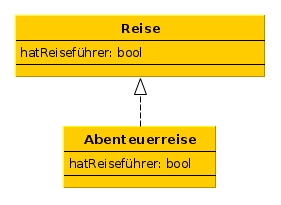
\includegraphics{bilder/experten_systeme_vererbung.png}}}
\caption{Einfaches Beispiel der Vererbung von Eigenschaften.\label{fig:experten_systeme_vererbung}\protect\footnotemark}
\end{figure}

\footnotetext{Eigene Darstellung mittels yEd.}

\noindent\rule[1ex]{\textwidth}{1pt}
\begin{wrapfigure}{l}{0.1\textwidth}
    \vspace{-14pt}
    
\includegraphics[width=0.1\textwidth]{bilder/owl.png}
\end{wrapfigure}
Eine Reise hat einen Reiseführer. Definiert man, eine Abenteuer-Reise ist auch eine Reise, ist es für den Menschen klar, dass eine Abenteuer-Reise auch einen Reiseführer haben kann. Beim Computer hingegen, muss die Unterklasse ``Abenteuer-Reise'' zuerst die Eigenschaft der Möglichkeit eines Reiseführers von der Oberklasse erben.\\

\noindent\rule[1ex]{\textwidth}{1pt}

\subsection{Prozedurales Wissen}
\label{subsec:prozedurales_wissen}
Bei prozeduralem Wissen handelt es sich um ein Wissen, welches in bestimmten Situationen bestimmte Aktionen vorschreibt. Man kann dies auch als Folge von Aktionen auffassen. So zum Beispiel das Aufschliessen einer Türe: Man steckt den (passenden) Schlüssel in das Schlüsselloch, dreht diesen, entsichert damit das Schloss, drückt die Türfalle nach unten und öffnet die Türe.

\begin{figure}[htbp]
\centering \rotatebox{0}{\scalebox{0.34}[0.34]{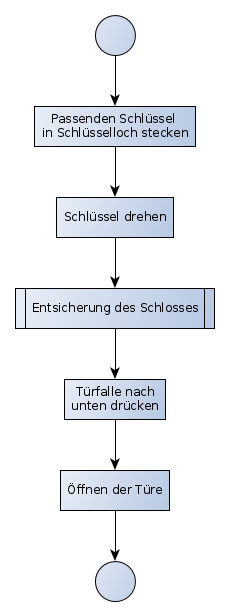
\includegraphics{bilder/experten_systeme_prozedurales_wissen.png}}}
\caption{Einfaches Beispiel von logischem Wissen.\label{fig:experten_systeme_prozedurales_wissen}\protect\footnotemark}
\end{figure}
\footnotetext{Eigene Darstellung mittels yEd.}

\newpage

\subsection{Logisches Wissen}
\label{subsec:logisches_wissen}

Bei logischem Wissen geht es im Grunde genommen um eine logische Implikation. Aus $A$ folgt $B$ bzw. $A \to B$, was so viel heisst wie ``Wenn $A$ gilt, kann geschlossen werden, dass auch $B$ gilt.''.

\noindent\rule[1ex]{\textwidth}{1pt}
\begin{wrapfigure}{l}{0.1\textwidth}
    \vspace{-14pt}
    
\includegraphics[width=0.1\textwidth]{bilder/owl.png}
\end{wrapfigure}
Möchte man darstellen, dass ein Ausflug teambildend ist, müssen folgende Voraussetzungen erfüllt sein: Für eine gewisse Anzahl Teilnehmer geeignet und gute Zusammenarbeit fördernd.

Formal ausgedrückt: $A \wedge B \rightarrow C$. Hierbei beudetet $A$: geeignet für eine gewisse Anzahl Teilnehmer, $B$: Förderung der Zusammenarbeit und $C$: ist teambildend.\\

\noindent\rule[1ex]{\textwidth}{1pt}

\section{Wissensrepräsentationsformalismen}
\label{sec:wissensrepräsentationsformalismen}
Sofern nicht anders vermerkt, basiert der folgende Abschnitt auf~\cite[S. 32]{laemmel}.

Formalisiert man die unter~\ref{itm:wissensarten} genannten Arten des Wissens, so gelangt man zu den folgenden Wissenrepräsentationsformalismen:
\begin{itemize}
    \item Logik
        \begin{itemize}
            \item Aussagenlogik
            \item Prädikatenlogik erster Stufe
        \end{itemize}
    \item Semantische Netze und Schemata (Frames)
    \item Regelbasierte Sprachen
\end{itemize}

Wie unter~\ref{sec:experten_systeme_komponenten} beschrieben, bildet die Basis eines Expertensystemes unter anderem eine Wissensdatenbank. Zur Erleichterung des Aufbaus einer Wissendatenbank und zur grafischen Darstellung, eignen sich Graphen sehr gut. Diese werden im nachfolgenden Kapitel beschreiben.
